%%%%%%%%%%%%%%%%%%%%%%%%%%%%%%%%%%%%%%%%%%%%%%%%%%%%%%%%%%%%%%%%%%%%%%%%%%%%%%%%
%                                                                              %
%	File:     introduction.tex                                                 %
%   Document: XXX	                                                           %
%   Author:   Freismuth David                                                  %
%	Date:	  22.JUN.2018                                                      %
%   Content:  Contains the Introduction section of the Bachelor thesis.        %
%                                                                              %
%%%%%%%%%%%%%%%%%%%%%%%%%%%%%%%%%%%%%%%%%%%%%%%%%%%%%%%%%%%%%%%%%%%%%%%%%%%%%%%%

%%%%%%%%%%%%%%%%%%%%%%%%%%%%%%%%%%%%%%%%%%%%%%%%%%%%%%%%%%%%%%%%%%%%%%%%%%%%%%%%
\section{Introduction}
As Embedded Systems find their way in an increasingly wide field of applications,
with growing demands to performance and relieability, the underlying Hardware 
Designs also gain in diversity, complexity and size. Since it is nearly impossible,
even for simple Designs, to determine the function of such, without proper
documentation, a possibility to extract information directly from the Hardware 
Description Language representation of the Design, seems to be a welcome aid.
Such a hardware design classification algorithm also allow services, which 
automatically handle aforementionend designs (for instance online sharing 
plattforms like gls{oc}) to assign categories without relying on user input.

\begin{figure}[h]
 \centering
 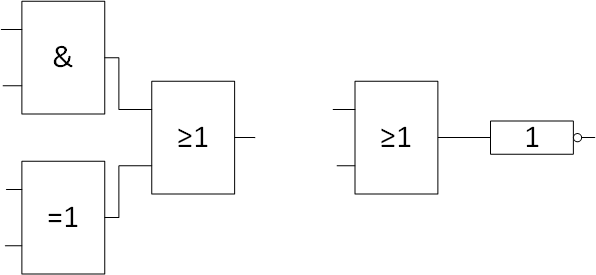
\includegraphics[width=\textwidth,keepaspectratio]{fig/logicGates.png}
 \caption{Example of a Two to One Connection (left) and an One to One Connection (right).}
 \label{fig:logicGates}
\end{figure}

This work tries to achieve a classification of hardware designs by analyzing the 
connection between logical cells. The count of specified two to one and one to 
one connections (examples depictioned in illustration), are translated into a
standardized match vector. It is expected that the match vector of similar designs
gather in clusters. These clusters can then be understood as hardware categories. 
Using a methodolodgy like this implies, that the location and meaning of those clusters first 
have to be identified, by analyzing a great amount of well known hardware designs.
The clustering is also in scope of this work, and is achieved by a web crawler,
which gathers already categorized designs from the open source sharing plattform 
gls{oc}. These designs are then synthesized by the open source synthesis tool 
gls{yosys} and handed over to the match algorithm, which eventually determines 
the match vector. The so gathered set of match vectors are then grouped into clusters.

The result of this work is a <command line application> which is able to 
categorize large designs (XXX Cells) in X seconds with a certainty of Y%.
The following chapters elaborate on the development, set of problems and 
other possible applications of this work. 
  
